\documentclass[12pt]{article}

%% Language and font encodings
\usepackage[english]{babel}
\usepackage{multirow}

%% Sets page size and margins
\usepackage[a4paper,top=3cm,bottom=2cm,left=3cm,right=3cm,marginparwidth=1.75cm]{geometry}

%% Useful packages
\usepackage{graphicx}
\usepackage[colorlinks=true, allcolors=blue]{hyperref}
\usepackage{setspace}   %Allows double spacing with the \doublespacing command
\usepackage{indentfirst}

\title{Askie Forum}
\author{
         Danh Nguyen\\
         \texttt{Onid:nguydanh}\\
         \texttt{nguydanh@oregonstate.edu}
         \and
         Joshua Bell\\
         \texttt{Onid:belljos}\\
         \texttt{belljos@oregonstate.edu}
         \and
         Cameron Kocher\\
         \texttt{Onid:kochecam}\\
         \texttt{kochecam@oregonstate.edu}
         \and
         Nicholas Newell\\
         \texttt{Onid:newelln}\\
         \texttt{newelln@oregonstate.edu}
         \and
         Andrew Morrill\\
         \texttt{Onid:morrilan}\\
         \texttt{morrilan@oregonstate.edu}
         \and
         GitHub: https://github.com/hydra314/AskieForum
    }

\begin{document}
\maketitle

\tableofcontents
\section{Project Description}
\begin{enumerate}
    \item \textbf{What is your approach? Who are the target users you expect to use your proposed solution, and what problem does it solve?}

        Our target users are specifically college students and business representatives at conventions. Since Askie Forum is a solution that is only available to users who carry an electronic device, our market will consist mainly of adults because of their ability and willingness to use electronic devices. What Askie Forum can do for these users is provide a comfortable environment where they can exchange questions and obtain quick responses instead of being afraid to obtain these answers due to a fear of public speaking. Askie Forum will provide a comfortable environment for its users by making them anonymous while also providing incentives for other users to answer questions.
    
        
    \item \textbf{State the key difference between your approach and previous approaches.}

    Askie Forum operates in the Educational Technology market, as it uses technology for the purpose of furthering education. Our main competitor will be Piazza, which is a free online gathering place where students can ask, answer, and explore under the guidance of their instructors. However, our software approach differs from Piazza's in numerous ways. While Piazza helps students obtain clarification, tips, and answers outside of class, Askie Forum allows students to do this in real time during lecture. When an instructor creates a forum to be used during lecture, all of the instructor's students will be able to access the forum and ask questions. Let’s say you are a user who has a question about something your professor is currently talking about in lecture. When you post the question on the forum, your question may be answered by anyone in the class. Fortunately,  when you're in class, you're within a pool of active users (including your instructor) who can help you out - whether with clarification, hints, resources, or the solution itself. With Piazza, users can ask questions and obtain answers in the same manner, but Piazza is not designed to be used during class; rather, its design lends itself to being useful outside of class. Therefore, it's not as easy to receive an answer since not everyone is on at the same time. 
    
    \item \textbf{Can you use a diagram to show how your approach plugs into existing resources?}
    
    
\includegraphics[width=\textwidth]{Assignment_2_ProjectDescription1}
    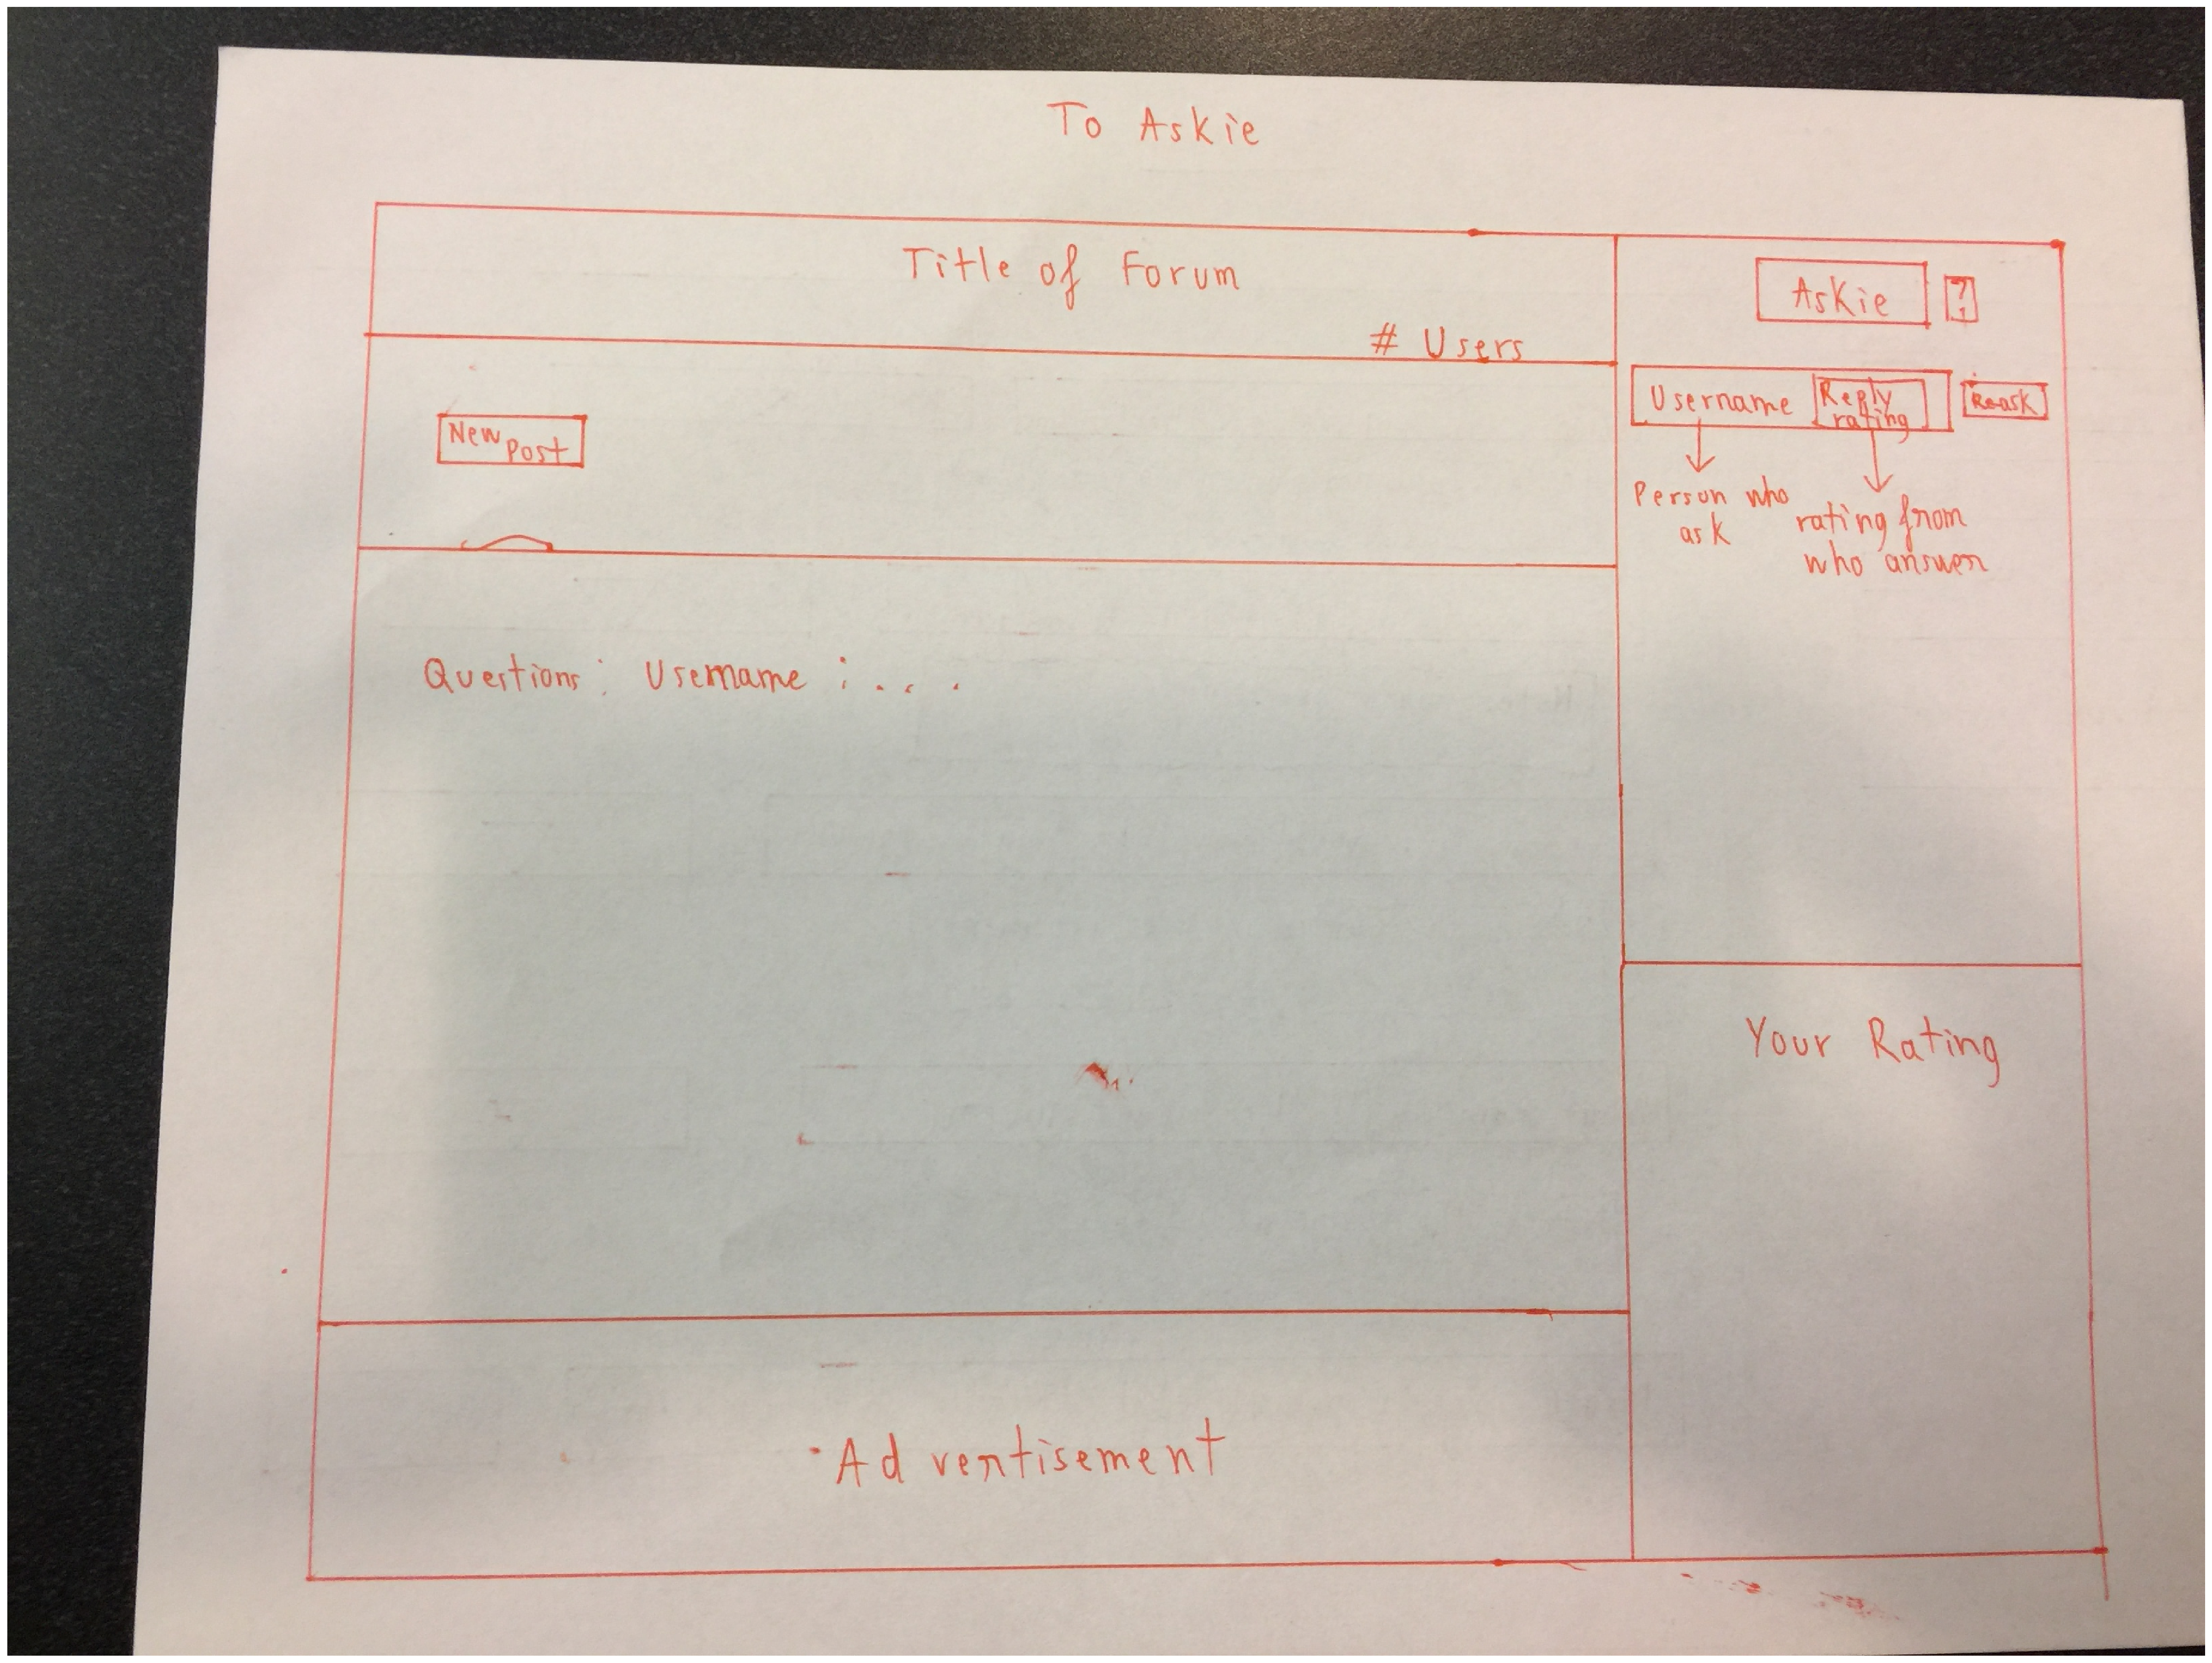
\includegraphics[width=\textwidth]{Assignment_2_ProjectDescription2}

    \item \textbf{What programming languages, and other tools will you use? Why have you chosen these languages and tools?}

    Meteor is a great software application for web, mobile, and desktop. It also has a lot of documentation as well as tutorials where we can obtain information. The programming language we will use will be Java Script, with MongoDB serving as our database. 

    \item \textbf{What are its functional requirements?}
\begin{itemize}
\item To use Askie Forum, there must be a host who creates the forum.
\item Questions that are marked as urgent must be answered before any other questions can be posted.
\item If the host answers the question, then the user who asks the question must mark it as having been answered in order to be able to continue asking questions.
\item Each user will be given a certain number of lives that represent how many stupid questions they may ask. If they run out of lives, they will not be able to enter the forum.
\item If a question marked as urgent is not answered within a certain timeframe (the timeframe will be set by the student asking the question), the host will be notified. The host must either answer the question immediately or set the question to be answered at the end of the forum.
\item For every question that is asked, the student asking the question can mark themselves as anonymous or not. Person who answer can also choose to mark themselves as anonymous if they feel as if their answers aren't good. 
\item A user must mark their question as answered if they are satisfied with the solution. Once the question has been marked as answered, it will be transferred over to a different section call Askies, which is an archive that stores all asked and answered questions.
\item There will be a re-ask feature that will allow users to reiterate a question. The user will be obligated to comment on why they are asking the question again.
\end{itemize}

    \item \textbf{What are its non-functional requirements?}
\begin{itemize}
\item Users can rate a given answer. This can be used for credibility purposes.
\item Questions will be labeled red, while answers will be labeled green.
\item A five star rating system will be used.
\item Sample expressions will be provided that may be used for certain subjects. This will help students write clear and concise questions.
\end{itemize}

    \item \textbf{What other documentation will you provide to help users understand and use your system? Documentation includes materials such user manuals, help buttons/texts throughout the user interface, etc.}

\underline{Documentation For The Host}

When someone would like to host a forum, they will be given the opportunity to go through the process of setting up their environment. This process will include questionnaires on how the host plans to deal with urgent questions, how many lives they would like to give to each user, what the subject of the forum will be, who is allowed to act as a host for the forum, the range that the event is covering, and what the passcode is for users who would like to join the forum. 

\underline{Documentation For The User}

When users log into their accounts, their home page will display a list of nearby events that they can join. To join a forum, they must have the forum's passcode given to them by the host. Once they join, they will be run through the environment specified by the host, and a built-in tutorial will walk them through the important points of the process, such as how many lives they have, how the host will answer urgent questions, how questions are created, and other useful things that will help teach them how to effectively use the software.

    \item \textbf{What are the major features of the system that make it so effective or useful? Include at least four major features you will provide, along with at least two features you hope to implement.}

\underline{Major features}
\begin{itemize}
\item The ability for users to mark their question as anonymous.
\item The ability for users to host a forum.
\item The ability for users to rate answers.
\item The ability for users to join a host's forum with a passcode. 
\end{itemize}

\underline{Features we hope to implement}
\begin{itemize}
\item Allow a user to host a forum.
\item Allow a user to join a forum.
\end{itemize}
\end{enumerate}

\section{Use Cases}

\subsection{Participation Optional}
\begin{itemize}
    \item \textbf{Name:} Participant Q/A
    \item \textbf{Goal}: Help participants answer questions about material 
    \item \textbf{Actors:} "Teachers", "Students", "TAs" (or equivalents)
    \item \textbf{Preconditions:} 
        \begin{enumerate}
            \item User has a computer
            \item User has internet connection
            \item Other people in the same course are using the site
        \end{enumerate}
    \item \textbf{Post-conditions:}
        \begin{enumerate}
            \item Question is posted
            \item Depending on the "mode", question may be posted as urgent
            \item Question may be answered
        \end{enumerate}
    \item \textbf{Flow of events:}
        \begin{enumerate}
            \item Actor logs into the site
            \item System verifies credentials
            \item The actor is presented with a list of events they are participating in, or a prompt to join/create a new event (event being a class, or some other form of presentation)
            \item On selecting an event, the actor is presented with questions that have been asked by other participants. "Urgent" questions are located at the top of the list, then unanswered questions, then answered questions.
            \item There should be a button to post a new question. Clicking on it will bring up a text box to submit it, as well as a checkbox for "Urgent" status.
            \item On selecting a question, the actor should be able to answer the question via a text box. Other answers should be visible.

        \end{enumerate}
    \item \textbf{Optional quality requirements:}
        \begin{enumerate}
            \item "Teachers" and "TAs" should be able to change the urgency of a question. Meaning, if a simple question is marked Urgent, they should be able to downgrade the urgency.
        \end{enumerate}
\end{itemize}

\subsection{Participation Required}
\begin{itemize}
    \item \textbf{Name:} Participation Required for Grading
    \item \textbf{Goal}: Provide a forum for participants to respond to lecture material
    \item \textbf{Actors:} "Teachers", "Students", "TAs" (or equivalents)
    \item \textbf{Preconditions:} 
        \begin{enumerate}
            \item User has a computer
            \item User has internet connection
            \item Other people in the same course are using the site
        \end{enumerate}
    \item \textbf{Post-conditions:} 
        \begin{enumerate}
            \item Answer is visibly posted as the "student" 
            \item “Teacher” should be able to differentiate between "students" answers
        \end{enumerate}
    \item \textbf{Flow of events:} 
        \begin{enumerate}
            \item Actor logs into the site
            \item System verifies credentials
            \item The actor is presented with a list of events they are participating in, or a prompt to join/create a new event (event being a class, or some other form of presentation)
            \item On selecting an event, the actor is presented with questions that have been asked by other participants. "Urgent" questions are located at the top of the list, then unanswered questions, then answered questions.
            \item Depending on implementation, there may be another question category required, marking it as "for grade"
            \item On selecting a question, the actor should be able to answer the question via a text box. Other answers should be visible.
        \end{enumerate}
    \item \textbf{Optional quality requirements:}
        \begin{enumerate}
            \item Depending on implementation, the "teacher" could be notified that the "student" has responded.
        \end{enumerate}
\end{itemize}

\subsection{Live Q/A}
\begin{itemize}
    \item \textbf{Name:} In-session Participation
    \item \textbf{Goal:} Aid student/teacher in-class exchanges by allowing a non-verbal communication option
    \item \textbf{Actors:} "Teachers", "Students", "TAs" (or equivalents)
    \item \textbf{Preconditions:}
        \begin{enumerate}
            \item User has a computer
            \item User has internet connection
            \item Other people in the same course are using the site
            \item Phones/computers are allowed during lectures
            \item "Teacher" has the application open
        \end{enumerate}
    \item \textbf{Post-conditions:}
        \begin{enumerate}
            \item question is posted
            \item Teacher may be notified that a question has been asked
            \item Question answered out loud, in person, or by text from other actors
        \end{enumerate}
    \item \textbf{Flow of events:}
        \begin{enumerate}
            \item Actor logs into the site
            \item System verifies credentials
            \item The actor is presented with a list of events they are participating in, or a prompt to join/create a new event (event being a class, or some other form of presentation)
            \item On selecting an event, the actor is presented with questions that have been asked by other participants. "Urgent" questions are located at the top of the list, then unanswered questions, then answered questions.
            \item There should be a button to post a new question. Clicking on it will bring up a text box to submit it, as well as a checkbox for "Urgent" status.
            \item Any actor may respond, but this enables "teachers" to respond to questions within a lecture, while not interrupting the flow
        \end{enumerate}
    \item \textbf{Optional quality requirements:}
        \begin{enumerate}
            \item ”Teacher” may be notified that a question has been asked.
        \end{enumerate}
\end{itemize}

\subsection{Justification}
    Due to the very nature of this application, the potential scope is rather small. This is something that will primarily be used in classrooms, guest lectures, or Q/A venues. These are all events where there is one or more orators (the "Teacher"), potentially some moderators (the "TAs"), and the guests (the "Students") being spoken to. As an app designed to encourage discussion between those guests, and allowing for answers from orators or moderators, there is little possible deviation. In a classroom scope, it is quite likely that the Required Discussion will come up at least once. Any venue can utilize optional discussion, though university students in particular are heavily impacted. There are many students who are either quite shy, who don't speak English as a primary language, or who have a disability that hinders in-class discussion. And while classrooms may not often utilize a live Q/A system, there are use cases for any other venue which relies on orators being asked questions.

\subsection{Error scenarios and possible solutions}
    \begin{itemize}
        \item Blank title for Forum name
            \begin{itemize}
                \item A dialog box should alert the user if they attempt to create a forum without a name, and prevent its creation.
            \end{itemize}
        \item Empty question body
            \begin{itemize}
                \item If the question has a separate title and body, a confirmation box should ask the user if they really want to post a question without a body. In this case, as above, a dialog box should prevent the creation of a question with no title OR body.
                \item If the question has only a body section, a dialog box should alert the user and prevent the creation of a question with no body.
            \end{itemize}
        \item Bad login
            \begin{itemize}
                \item A generic "cannot log in" message should be given to the user. You should NOT tell them specifically if the username or password was wrong.
            \end{itemize}
        \item Bad Forum passcode
            \begin{itemize}
                \item An error message should tell the user that "The forum either does not exist yet, or the passcode used is wrong", and that they should check with the forum creator.
            \end{itemize}
        \item 404
            \begin{itemize}
                \item A "Page not Found" screen should be displayed instead, and a link to the Home Page should be easily accessible
            \end{itemize}
        \item Forum already exists
            \begin{itemize}
                \item An error indicating that the forum name is already in use should be given to the user. Forum creation should fail.
            \end{itemize}
        \item Database unreachable
            \begin{itemize}
                \item An error indicating that the site back end is down should appear centrally in the Home Page. 
            \end{itemize}
    \end{itemize}


\section{Planning}
\subsection{Milestones}
\begin{flushleft}
Large milestones would include creating a database to keep track of all the login information, forum posts, etc. The next would be getting the basic site functions and layout to work. The final milestone would include making the interface look nice and adding last minute features to make the user experience a little nicer.
\end{flushleft}
\subsubsection{Database:} 
\begin{flushleft}The database will allow users to create accounts that will contain information about, among other things, their name, major, and contact information. The database will keep track of the user's rating as well as what questions they have asked and answered. It will also keep track of their personal Askie Forum settings, such as their urgent question priority.
\end{flushleft}
\begin{flushleft}

\subsubsection{Basic Layout and Functionality:}
\begin{flushleft}The basic forum layout and functions will link and communicate with the database. It will be partially worked on alongside - but will be finished after - the database, as it requires the database to be functional. It will also lead up to the final milestone.
\end{flushleft}
\begin{flushleft}
The final milestone will involve making the website look appealing to the userbase and adding any last minute features. This is basically a buffer - if the schedule fails, this milestone will likely be at least partially cut.
\end{flushleft}

\subsection{Tasks}
\end{flushleft}
\subsubsection{Entity Relationship Diagram (ERD):} 
\begin{flushleft}Constructing an Entity Relationship Diagram will be a crucial step in the process of designing the project in general. We will split into sub-teams in order to facilitate the creation of the database alongside the design of the layout. Having a clear ERD makes constructing the database far easier, as we'll more easily be able to identify the relevant entities and relationships. This will be the first vital step in completing the database design, and it will also help solidify the user-entered information on the forum. 
\end{flushleft}
\subsubsection{Site Map:} 
\begin{flushleft} The site map will be worked on side-by-side with the ERD. It will outline the basic layouts of the forum pages, and will make life far easier for the group members tasked with writing the HTML and CSS for the site.
\end{flushleft}
\subsubsection{Implement Database:} 
\begin{flushleft}Implementing the database will be a crucial early step in the life-cycle of this project. Having a working database is necessary for when we start testing communication with the forum; without a functional database, creating core components such as user logins and forum posts will be impossible. If we have any bugs in the database, we can catch them early on, as not having the database linked with anything will make issues far easier to detect.
\end{flushleft}

\subsubsection{Basic Layout (HTML):} 
\begin{flushleft}This task will involve laying out basic versions of important forum pages while also discussing how they should interconnect. This will be done primarily in HTML and CSS, and it should reflect design choices made earlier. This lays the groundwork for the next task.
\end{flushleft}

\subsubsection{Basic Login Screen:} 
\begin{flushleft} A login screen will allow us to test the functionality of our database. Additionally, it will allow users to create and use personal accounts.
\end{flushleft}

\subsubsection{Basic User Interface:} 
\begin{flushleft} The user interface will make the site usable. It will involve the following: giving users the ability to post question threads; giving users the ability to respond to posts on threads made by themselves or others; giving users the ability to modify their personal details; creating flags and labels, such as "Urgent"; and essentially giving form to everything else that has already been created and implemented so that they can be used and interacted with. Most of this task will be done in Javascript.
\end{flushleft}

\subsubsection{User-Forum Interaction:} 
\begin{flushleft} This is a large part that should mostly consist of allowing users to create forums and communicate between each other. This will have to be done side by side of User Security, with final implementation with our database interactions prioritized first, so User Security can be finished on time as well.
\end{flushleft}

\subsubsection{User Security:} 
\begin{flushleft}Privacy is a major concern in today's Internet age, so implementing user confidentiality will be mandatory if Askie Forum is to have any credibility. Like any other login-based website, we will use encryption and online security services to provide privacy to users and allow their information to be protected from being modified by other user. It will be implemented near the end of production, after the main features are complete. However, the website should not go live before security is implemented.
\end{flushleft}
\subsubsection{Make Everything Pretty:} 
\begin{flushleft}   
The final task, if we have time, this is what we will be spending the last of the term on.  Making it nicer and more appealing for users to navigate and to view.
\end{flushleft}

\subsection{Schedule}
% Please add the following required packages to your document preamble:
% \usepackage{multirow}
\begin{table}[!h]
\centering
\caption{My caption}
\label{my-label}
\begin{tabular}{|l|c|c|c|c|}
\hline
\textbf{Time Frame} & \textbf{Task 1}                         & \textbf{Task 2}                & \multicolumn{1}{l|}{\textbf{Meeting \#1}}                                                                   & \multicolumn{1}{l|}{\textbf{Meeting \#2}}                                                             \\ \hline
1/29 - 2/05         & ERD                                     & Design Site Map                & \multirow{7}{*}{\begin{tabular}[c]{@{}c@{}}Saturday\\ 1 pm,\\ Library\\ (Subject to\\ Change)\end{tabular}} & \multirow{7}{*}{\begin{tabular}[c]{@{}c@{}}Anytime\\ during week\\ days,\\ Kelly Atrium\end{tabular}} \\ \cline{1-3}
2/6 - 2/12          & \multirow{2}{*}{Implement Database}     & Basic Layout HTML              &                                                                                                             &                                                                                                       \\ \cline{1-1} \cline{3-3}
2/13 - 2/19         &                                         & Create Basic Login             &                                                                                                             &                                                                                                       \\ \cline{1-3}
2/20 - 2/26         & \multicolumn{2}{c|}{Basic User Interface}                                &                                                                                                             &                                                                                                       \\ \cline{1-3}
2/27 - 3/06         & \multirow{2}{*}{User-Forum Interaction} & \multirow{2}{*}{User Security} &                                                                                                             &                                                                                                       \\ \cline{1-1}
3/07 - 3/14         &                                         &                                &                                                                                                             &                                                                                                       \\ \cline{1-3}
3/15 - 3/22         & \multicolumn{2}{c|}{Make Everything Pretty}                              &                                                                                                             &                                                                                                       \\ \hline
\end{tabular}
\end{table}
\subsection{Project Tracking}
\begin{flushleft}We will keep keep track of our progress by taking time to look back at the goals we have set and evaluating the degree to which those goals have been accomplished. By setting specific goals and identifying the individual tasks we need to complete in order complete this project, we will always be aware of the progress we have made, and we will be able to predict how quickly we will need to progress to meet the deadline.
\end{flushleft}
\begin{flushleft}
In addition to tracking our progress, we will also need to ensure that the quality of our work is up to par. We will be able to accomplish this by setting standards for each of the individual tasks as well as the project as a whole. At any time throughout the project, we can compare our work to the standards we have set so we are always aware of the quality of our work.
\end{flushleft}
\subsection{Risk Management}
\begin{flushleft}
The main risks that we anticipate are ones that are common to every software development project. These include, but are not limited to, the following: members not being familiar with a programming language, members being unable to participate (whether due to time constraints, illness, or other factors), and possible computer trouble.
\end{flushleft}
\begin{flushleft}
Members not being familiar with a specific programming language is a risk, as another member may need to allocate time to teach the other member how to code in that language. To minimize this problem, we will divide work based off of who can do what. For example, one of our members isn't very strong in CSS but excels at HTML; that member will therefore work mainly on the website's layout, while leaving CSS styling to the other members.
\end{flushleft}
\begin{flushleft}
Another risk that we must take into account is computer trouble. Sometimes software doesn’t work on one computer the same way it works on others, causing members to have to spend time debugging rather than working on the project. The absolute worst-case scenario would involve a group member's hard drive crashing. In which case, not only would we need a replacement computer for that member, we would lose anything stored on their original hard drive. To prepare for the worst possible computer problems, we will keep backups of everyone's work - these will mainly be stored on GitHub, but flash drives and/or external hard drives may be used if the situation calls for them. A quick backup every night will prevent us from losing too much data in the event of a catastrophic hardware malfunction. The member whose computer lost its functionality would likely have to do all their work at school, where they would use the university’s computers to keep up on their work.
\end{flushleft}
\begin{flushleft}
The largest risk probably resides in poor communication. It makes group meetings harder to schedule, it can lead to lost efficienty, and it may cause members to have to redo parts of the project. Negative, unhelpful criticism may also pose a problem, as not only can it potentially cause huge wastes of time, it can cause members to dislike each other in the end. To prevent this, we will have to be able to be easily reachable and flexible. The design and schedule must be laid out nicely so that everyone knows what is coming up and what needs to be done by a certain date.
\end{flushleft}
\section{Meeting Report}
\begin{flushleft}
During this week we were able to get started on the project by beginning the planning process. Most of the group was able to meet in person, so we were able to get acquainted with those whom we will be spending the next few weeks working on this project with. By meeting together, we were able to solidify our ideas of the project so that we could develop specific tasks needed to successfully get the project done.
\end{flushleft}
\begin{flushleft}
Though we are still in the early stages, we were able to put a plan in place so that we can complete the project as efficiently as possible. In the next week we will begin working on the database that our application will use. By the end of the of the week we will have the ER diagram designed and will have developed a site map.
\end{flushleft}
We have assigned tasks to each group member so that the project and Assignment 2 are completed as efficiently as possible. Though we are all working on a single project, by splitting it up into subtasks, we are able to make use of everyone’s time at once.
\begin{flushleft}
Three of the five group members were able to meet in person, so they were the ones who made the decisions for the plan for the upcoming week. One of the two customers was able to come to the meeting, but both will be able to come to subsequent meetings in the upcoming week.
\end{flushleft}



\end{document}
